\section{Séries Temporelles et Modèles de prédiction}
\label{sec:modeles}

Commençons par rappeler le format de données actuel. Nos données sont un ensemble de séries temporelles, par jours, du nombre de ventes par produit sur une période de 5 ans, de A14 à P19. Elles sont stockées dans un DataFrame de la bibliothèque python \emph{pandas}. Une colonne correspondant à un produit, identifié par son ID et chaque ligne correspond à un jour de vente, comme présenté ci-dessus.
\begin{figure}[H]
    \centering
    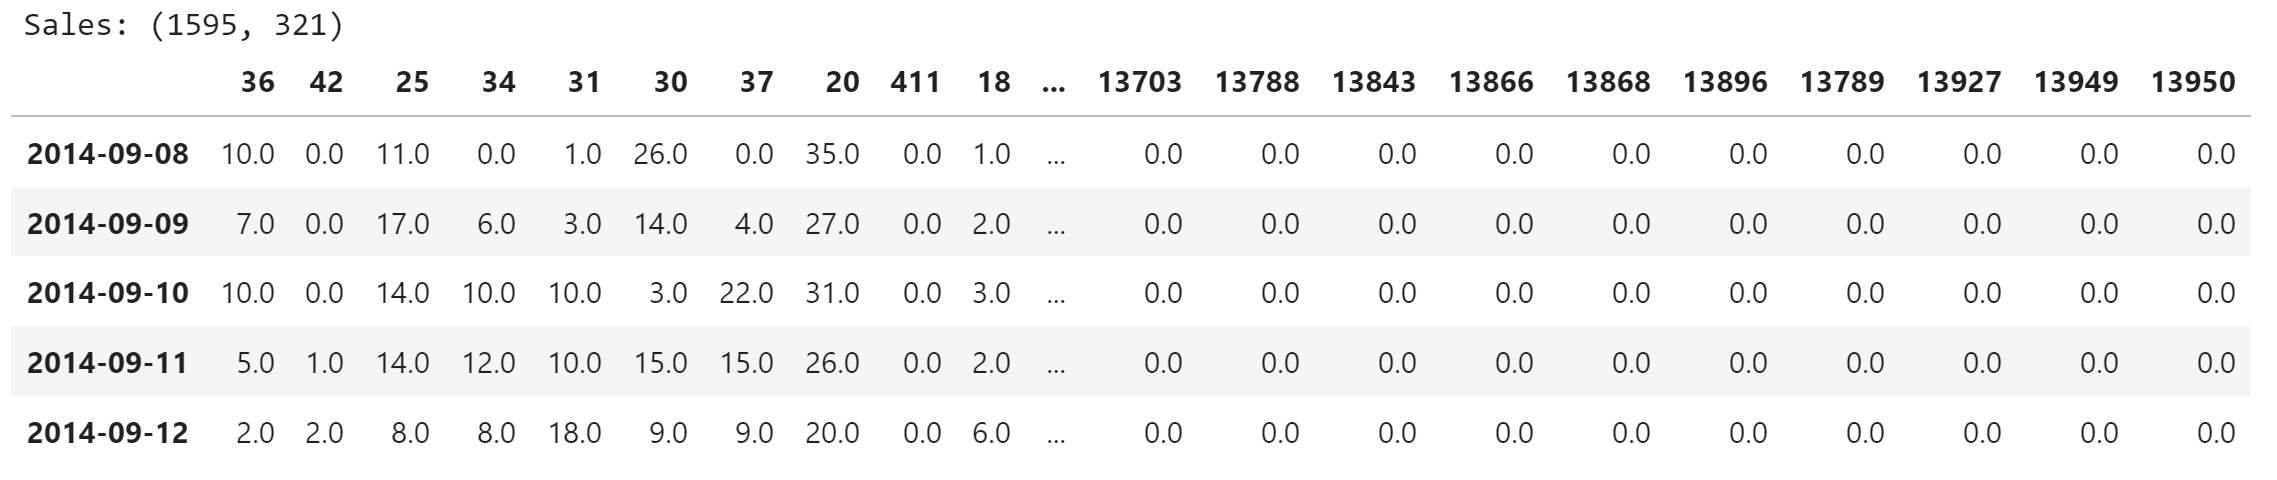
\includegraphics[width=\textwidth]{figures/sales_df.png}
    \caption{Aperçu du DataFrame des ventes}
    \label{fig:sales_df}
\end{figure}

Le but est de pouvoir prédire le nombre de vente des différents produits pour la semaine suivante. Pour cela on ne s'intéressera qu'à un ou deux produits pour tester nos modèles. Les résultats suivants correspondent donc aux modèles appliqués à deux produits : le Pampryl Abricot et le Café. Nous les avons choisis car ils sont vendus depuis le début des ventes collectées, sont peu sujet aux ruptures de stock qui seraient difficile à prédire et fausseraient les données.
Nous avons également réalisé les tests sur la vente de différentes bières mais les mauvais résultats nous ont poussé à nous retrancher sur des produits dont les ventes ont une moins grande variance et dépendant moins des évènements.

Pour le moment, nous faisons des hypothèses simplificatrices. On considérera par exemple que l'évolution des ventes d'un produit est indépendante de l'évolution des autres produits. Cela peut paraître faux à première vue puisque si les étudiants consomment un produit en particulier, ils consommeront moins un autre mais en prenant des produits tels que le café, produit d'habitué, l'hypothèse n'est pas absurde. On réalisera d'autres hypothèses au fur et à mesure de nos avancée.


\subsection{Analyse exploratoire des données}
\label{subsec:expl_data}

Pour chaque produit, nous avons donc le nombre de vente par jour. Dans un premier temps, on note que tous les jours ne sont pas présents. Ce sont les jours où nous n'avons aucune vente. Or, lors du tracé du nombre de ventes en fonction du temps, on remarque que les ventes sur les dates manquées sont interpolées linéairement alors que les ventes sont censées être nulles. Nous traitons rapidement ce problème en rajoutant les jours manquants au DataFrame avec un nombre de vente égal à $0$ ce qui fait plus de sens.

\subsubsection{Observation des ventes globales}

Commençons par observer les ventes du Pampryl Abricot et du Café sur tout la période disponible.
\begin{figure}[H]
	\centering
	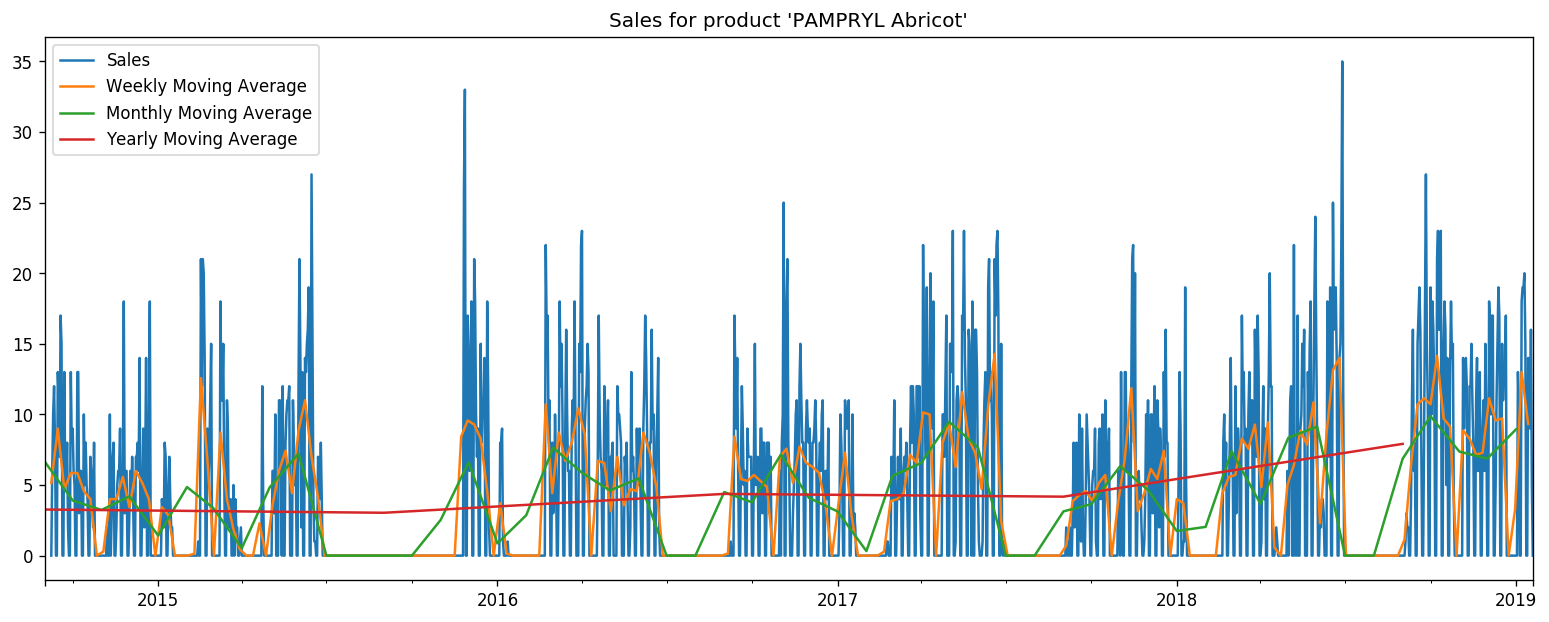
\includegraphics[width=\textwidth]{figures/all_sales_pampryl_abricot.png}
	\caption{Ventes du Pampryl Abricot}
    \label{fig:all_sales_pampryl_abricot}
\end{figure}

\begin{figure}[H]
	\centering
	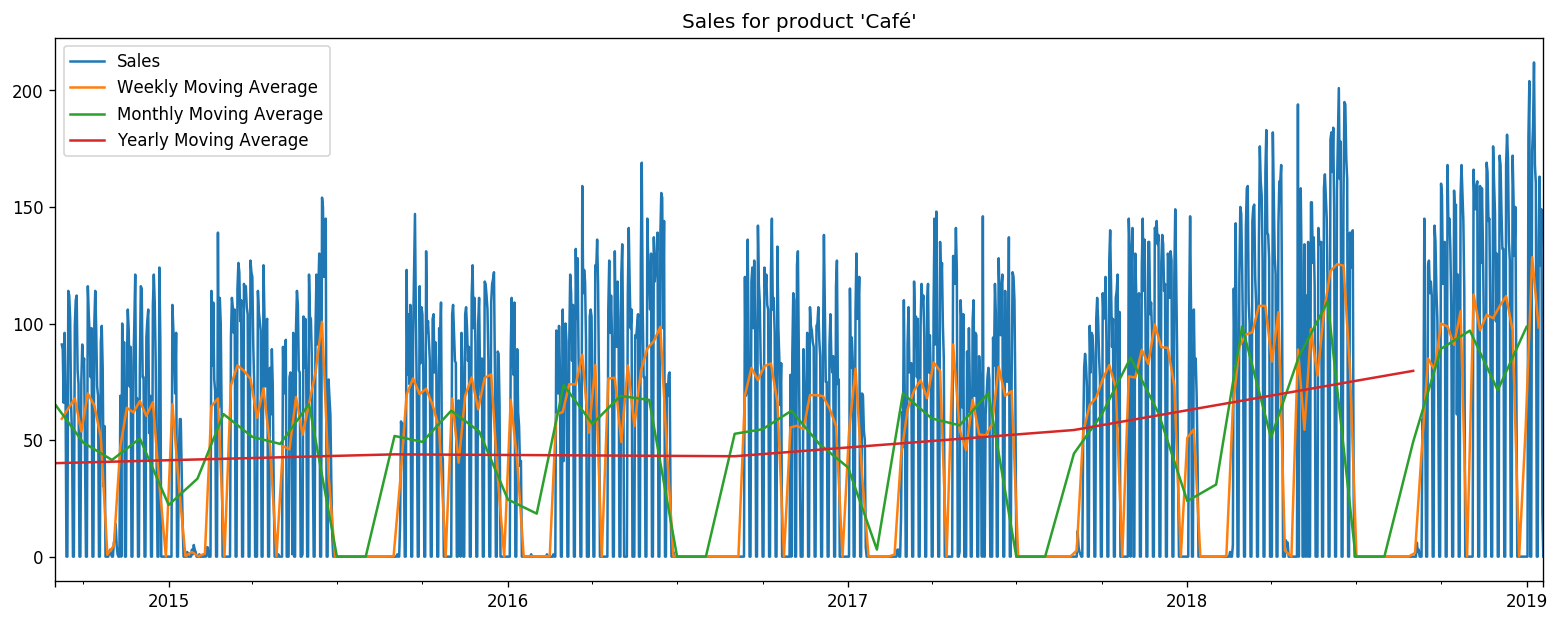
\includegraphics[width=\textwidth]{figures/all_sales_cafe.png}
	\caption{Ventes du Café}
    \label{fig:all_sales_cafe}
\end{figure}

Nous avons ajouté les moyennes par semaine, mois et années afin de mieux visualiser le comportement des ventes. Tout d'abord on observe bien sur les deux graphiques des ventes nulles lors des week-ends et des vacances, mais aussi des pics de ventes parfois au début, au milieu ou à la fin des semestres ainsi qu'une progression du volume de vente par semestre. On note aussi quelques différences: le Café est vendu en plus grandes quantités et varie moins que le Pampryl.

\subsubsection{Observation des ventes par semestres}

Pour un produit, par exemple ici le Pampryl, nous traçons les ventes en fonction du temps par semestre. Cela a pour but de mettre en évidence des comportements similaires entre les semestres, par exemple s'il y a plus de consommation à l'approche des vacances. On obtient alors le graphique si dessous.

\begin{figure}[H]
	\centering
	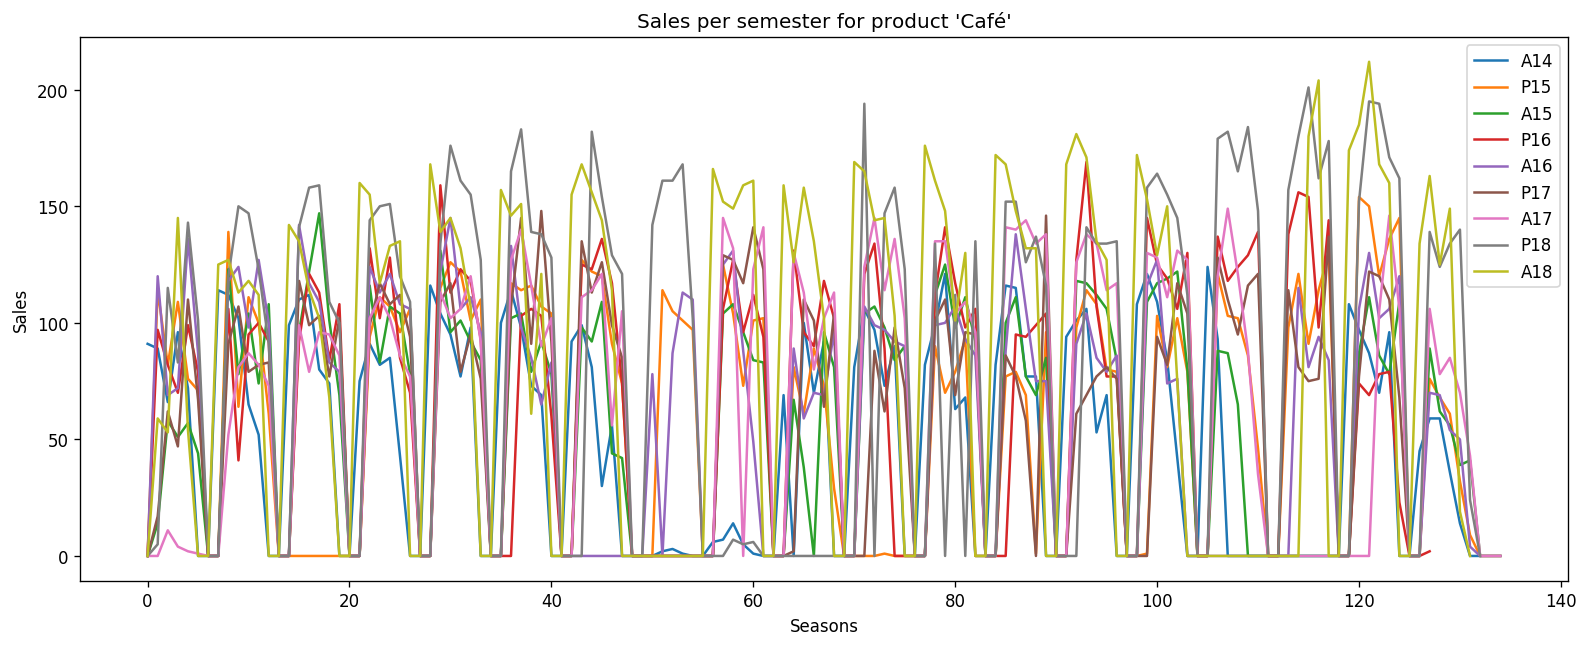
\includegraphics[width=\textwidth]{figures/sales_per_semester_cafe.png}
	\caption{Ventes du Café en fonction des semestres}
    \label{fig:sales_per_semester_cafe}
\end{figure}

On remarque qu'un schéma saisonnal se dessine, mais décalé différemment selon les semestres. Cela témoigne alors d'un problème majeur: les semestres n'ont pas tous le même format. Ces différences mineures vont compliquer la modélisation.
De plus, un semestre ce compose d'une multitude d'évenements. Ces évenements ne sont pas présents à tous les semestres et encore moins aux mêmes dates. Cela rajoute encore davantage de problèmes.


\subsection{Un premier test des modèles \ARIMA}
\label{subsec:arima}

Sans connaissance sur les séries temporelles, sur recommandation de nos encadrants nous avons commencé à étudier les modèles de type ARIMA. Le principe de tels modèles est de déterminer la valeur de la série à un instant $t_i$ en fonction des valeurs précédentes, c'est à dire aux instants $t_{i-1}$, $t_{i-2}$, ... Pour la suite nous prendrons les ventes de Café \ref{fig:all_sales_cafe} comme série temporelle notée \ts.

\subsubsection{Le modèle \ARIMA}

\ARIMA signifiant \emph{AutoRegressive Integrated Moving Average} est un modèle de prédiction de séries temporelles composé de plusieurs modèles.

La partie \emph{AutoRegression} indique que le modèle comporte une régression par rapport à la série en elle même. Le modèle $\AR(p)$ est paramétré par $p$ le nombre de retards pris en compte. On a alors:
\begin{equation}
    \AR(p) : x_i = c + \epsilon_i + \sum_{k=1}^p \phi_k x_{i-k}
    \label{eq:ar}
\end{equation}
avec $x_i$ la valeur de la série à l'instant $i$, $(\phi_k)_{k=1..p}$ les paramètres du modèles et $\epsilon_i$ un bruit blanc.

Un bruit blanc $\epsilon$ est une variable aléatoire telle que:
\begin{equation}
    \begin{cases}
        E(\epsilon_i) = 0             & \forall i \\
        E(\epsilon_i^2) = \sigma^2    & \forall i \\
        E(\epsilon_i \epsilon_j) = 0  & \forall i, j
    \end{cases}
    \label{eq:white_noise}
\end{equation}

La partie \emph{Moving Average} indique que l'erreur de regression est une combinaison linéaire des erreurs précédentes. Le modèle $\MA(q)$ est paramétré par $q$ le nombre de retards pris en compte pour l'erreur. On a:
\begin{equation}
    \MA(q) : x_i = \mu + \epsilon_i + \sum_{k=1}^q \theta_k \epsilon_{i-k}
    \label{eq:ma}
\end{equation}
avec $(\theta_k)_{k=1..p}$ les paramètres du modèles et $\mu$ la moyenne de la série.

Enfin \emph{Integrated} indique que la série est différenciée. Pour $\model{I}(d)$, les valeurs la séries ont été remplacées par la différence entre la valeur à l'instant $i$ et à l'instant $i-d$.

Ces 3 composantes permettent de former un modèle complet $\ARIMA(p,d,q)$ où les paramètres correspond à ceux vus dans les modèles précédents. En revanche, ce type de modèle ne prend pas en compte la saisonnalité. Pour cela il faudra utiliser les modèles \SARIMA, variante d'\ARIMA sur lesquels nous reviendrons.

\subsubsection{Stationnarité}
\label{subsec:stationarity}

\ARIMA est paramétrable mais nécessite une série temporelle stationnaire. Une série temporelle $(x_i)$ est dite stationnaire (au sens faible) si:
\begin{equation}
    \begin{cases}
        E(x_i) = \mu                  & \forall i \\
        Var(x_i) = \sigma^2 < \infty  & \forall i \\
        Cov(x_i, x_{i-k}) = f(k)      & \forall i,k
    \end{cases}
    \label{eq:stationarity}
\end{equation}

Nous allons alors tester la stationnarité de notre série.

Nous avons commencer par le test \textbf{KPSS} (Kwiatkowski-Phillips-Schmidt-Shin) de la librairie \emph{statsmodel}. L'hypothèse $H_0$ de ce test est que la série est stationnaire. L'application d'un tel test à \ts pour une tendance constante ou linéraire nous donne une $p$-value de $0.1$. On ne peut donc pas rejeter l'hypothèse de stationnarité de notre série.

Puisque l'on ne peux pas conclure de la stationnarité autour d'une tendance, nous avons eu l'idée d'utiliser un autre test. Il n'existe pas à proprement parler de tests où l'hypothèse $H_0$ est la non-stationnarité de la série. Un test beaucoup utilisé dans ce cas est le test de \textbf{Dickey-Fuller augmenté}. L'hypothèse $H_0$ est que la série ne contient pas de racine unitaire et donc qu'elle n'est pas stationnaire. L'hypothèse est validée si la série ne varie que par un bruit blanc ($x_t = x_{t-1} + \epsilon_t$).
Nous obtenons les résultats suivants:
\begin{table}[H]
    \centering
    \begin{tabular}{|l|r|l|}
        \hline
        Tendance & $p$-value \\
        \hline
        constante (c)      & 1.035E-05 \\
        linéire (ct)       & 4.649E-05 \\
        quadratique (ctt)  & 1.769E-04 \\
        non constante (nc) & 6.602E-03 \\
        \hline
    \end{tabular}
    \caption{Résultats du test de Dickey-Fuller augmenté pour le Café}
    \label{tab:adf_results_cafe}
\end{table}
On rejette donc $H_0$, la série temporelle ne possède pas de racine unitaire et peut être stationnaire.

Ainsi, nous ne pouvons pas conclure sur la stationnarité de la série \ts. Nous pouvons quand même faire l'hypothèse qu'elle l'est et tenter d'appliquer le modèle \ARIMA et revenir sur les hypothèses si cela ne fonctionne pas.


\subsubsection{Choix des paramètres p, d, q}
\label{subsec:params_pdq}

Pour choisir ces paramètres, plusieurs méthodes existent:
\begin{itemize}
    \item Estimation graphique
    \item Recherche automatisée
\end{itemize}

\paragraph{Estimation graphique}
\label{par:pdq_plots}

Comme nous nous intéressons au nombre de ventes par jour et non à sa variation, nous fixons $d=0$. Pour trouver des valeurs de $p$ et $q$ adéquates, nous avons deux outils à notre disposition. Le graphique d'autocorrélation (ACF) et le graphique d'autocorrélation partielle (PACF).

L'ACF nous donne l'autocorrélation entre la série et ses différents retards. On peut trouver le nombre de retards dont dépend la série et ainsi lui associer l'ordre $q$ du modèle de la Moyenne Mobile.

Le PACF nous donne la corrélation entre la série et ses retards, non expliquée par les retards précédents. Cela nous permet de déterminer l'ordre $p$ du modèle d'autorégression.


Nous avons donc les graphiques suivants:
\begin{figure}
    \centering
    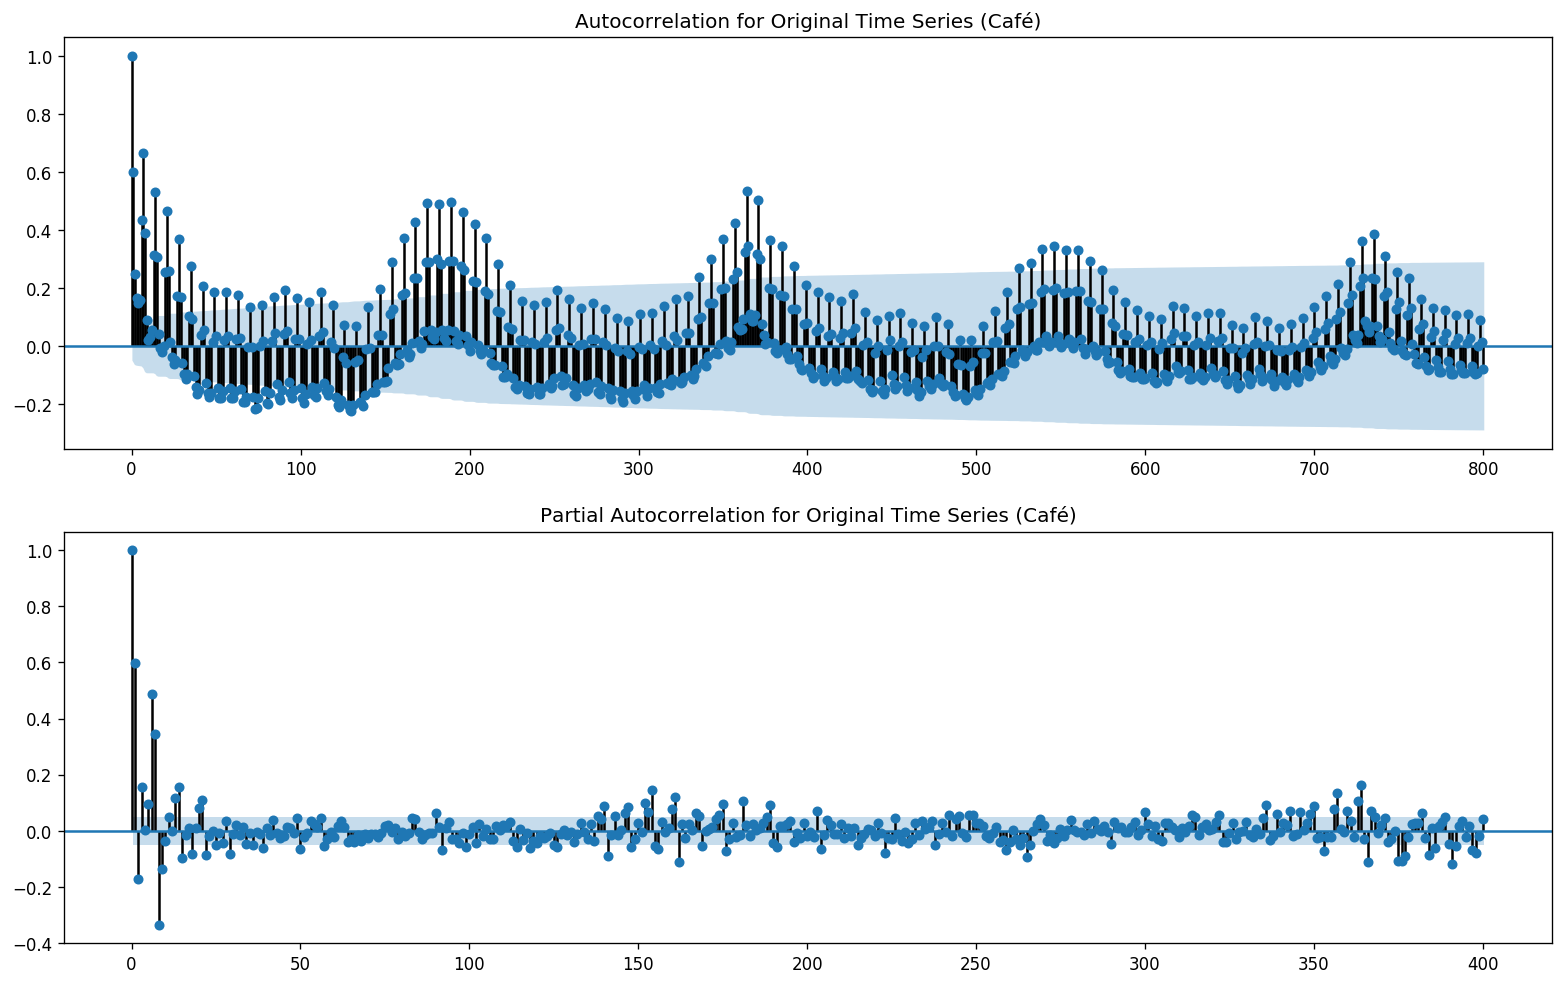
\includegraphics[width=\textwidth]{figures/acf_pacf_cafe.png}
    \caption{ACF et PACF de la série Café}
    \label{fig:acf_pacf_cafe}
\end{figure}

La zone bleu donne les autocorrélations non significatives à $95\%$.

On observe sur l'ACF une périodicité par semaine (tous les 7 retards) et une autre par semestre et année (tous les 182 et 365 retards). \ARIMA n'est pas capable de prendre en compte cette saisonnalité mais le modèle \SARIMA oui.

Nous avons donc tester \ARIMA avec toutes les combinaisons $p$ et $q$ égaux à $7$ et $182$. On remarque que le temps d'apprentissage est extrêmement long lorsque l'on utilise un ordre tel que $182$. Cela peut prendre plusieurs heures sans aboutir et ce n'est pas viable pour notre recherche et notre projet. Malgré cette recherche de paramètres, les résultats sont encore mauvais. C'est pourquoi nous sommes passé au modèle \SARIMA.

\paragraph{Recherche automatisée}
\label{par:grid_search}

% Dans un premier temps nous avons fait une recherche des différents paramètres en testant les différentes valeurs. Ces tests ont été fait d'abord à la main avec visualisation graphique de l'erreur entre les prédictions et les ventes réelles. Ensuite nous avons automatisé cela à l'aide d'une GridSearch.

La recherche automatisée consiste à définir une grille de paramètres à tester, puis de retenir la combinaison qui minimise un certain critère comme l'AIC (Critère d'information d'Akaike), le BIC (Critère d'information Bayésien) et la classique MSE (Erreur Quadratique Moyenne).

Pour cela nous avons d'abord créé la fonction \code{utils.models.ts\_grid\_search} qui effectue une recherche automatisée parallélisable avec des listes de valeurs pour les paramètres et un compte rendu détaillé des performances des modèles.
Puis nous avons découvert le package \code{pmdarima} qui propose la méthode \code{auto\_arima} recherche et donne le modèle optimisant l'AIC à partir d'intervalles de valeurs pour les paramètres.

Malgré ces différents indicateurs et ces différentes méthodes, nous n'avons pas trouvé de paramètres fonctionnels et encore moins optimaux. Lors de nos visualisations des résultats, les écarts entre les prévisions et les ventes étaient bien trop importantes.

\paragraph{Évaluation des performances}
\label{par:eval_perf}

Pour évaluer les performances d'un modèle de manière complète nous avons créé la fonction \code{utils.models.evaluate\_model}. Cette fonction facilement paramétrable prend un modèle entraîné, affiche les prédictions avec des indicateurs tels que AIC, BIC et MSE.

Pour les prédictions, deux méthodes sont possibles.
La première consiste à faire une seule prédiction directement pour tout le semestre: rapide mais très peu fiable sur la durée donc peu utile.
Le deuxième est un roulement de prédictions (\emph{rolling forecast}). Il s'agit d'une boucle apprentissage/prédiction qui permet avec des données de test, d'avoir une meilleure évaluation des performances du modèle sur la série temporelle. C'est la méthode qui sera appliquée en production pour prédire jour par jour ou semaine par semaine les ventes.
Le boucle est la suivante:
\begin{enumerate}[nolistsep]
    \item Apprentissage des données d'entraînement
    \item Prédiction d'une période (1 semaine ou 1 jour)
    \item Comparaison à la période réelle connue
    \item Ajout de la période réelle aux données d'apprentissages
    \item Ré-apprentissage du modèle avec les nouvelles données d'apprentissages
    \item Retour au point 2.
\end{enumerate}

Une étape supplémentaire serait de recalculer les paramètres optimaux après l'étape 5. Cela sera implémenter pour la production mais pour des raisons de rapidité de calculs nous ne le ferons pas dans nos expérimentations.

Ici nous utiliserons la méthode du roulement de prédictions avec comme données de test le semestre A18 entier.


\paragraph{Résultats}
\label{par:arima_results}

Le meilleur modèle \ARIMA obtenu avec \code{auto\_arima} a pour paramètres $(p=5, d=0, q=5)$. Avec la méthode décrite précédemment nous obtenons les résultats suivants.

\begin{table}[ht]
    \centering
    \begin{tabular}{r|r}
        AIC & 14436.25 \\
        \hline
        BIC & 14504.94 \\
        \hline
        MSE &  2401.85 \\
    \end{tabular}
    \caption{Résultats pour \ARIMA(5,0,5) sur le Café}
    \label{tab:pred_arima_cafe}
\end{table}

\begin{figure}[ht]
    \centering
    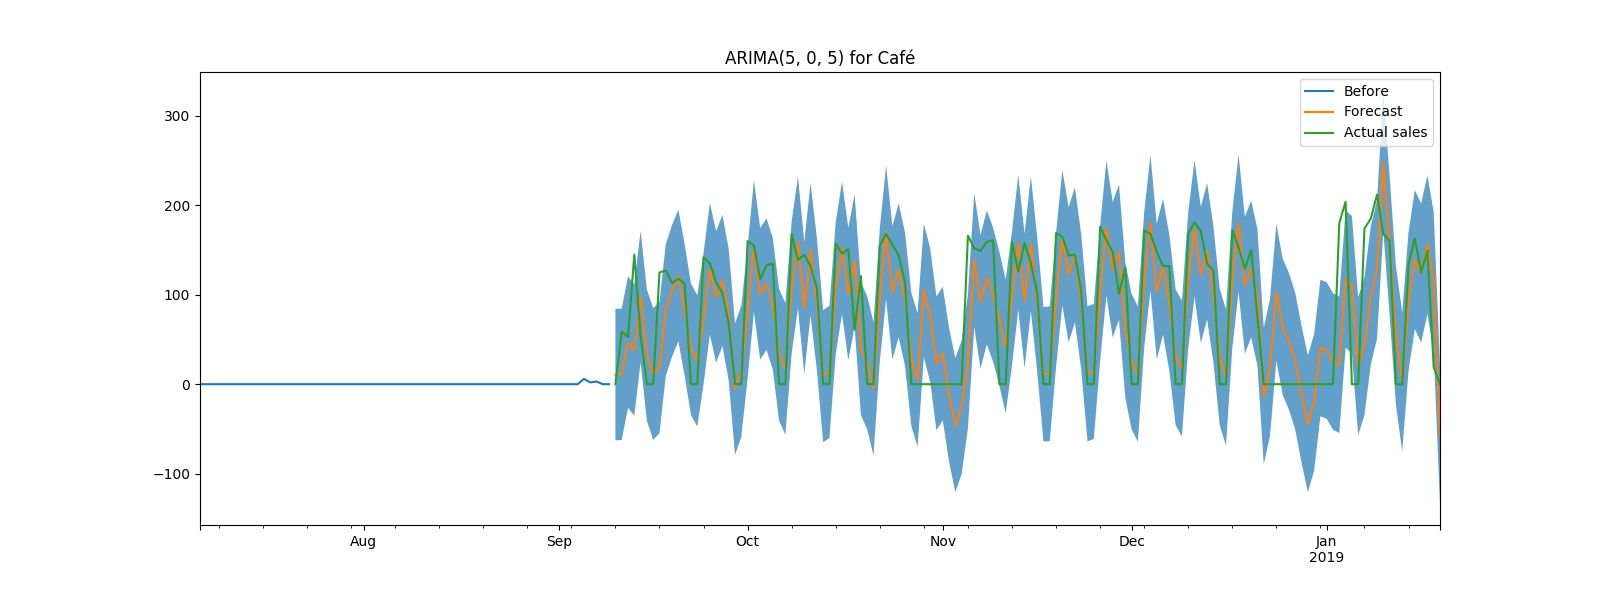
\includegraphics[width=\textwidth]{figures/pred_arima_cafe.jpg}
    \caption{Prédiction \ARIMA pour le Café}
    \label{fig:pred_arima_cafe}
\end{figure}

Les résultats semblent cohérents mais sont assez peu précis. Nous allons essayer d'exploiter la saisonnalité observée et d'ajouter des variables exogènes avec \SARIMAX pour améliorer les performances.


\subsection{Le modèle \SARIMAX}
\label{sec:sarimax}


\subsubsection{Le modèle \SARIMA, ajout de la saisonnalité}
\label{subsec:sarima}

\SARIMA est une variante du modèle \ARIMA comprenant une composante de saisonnalité. Nous avons désormais 4 paramètres supplémentaires:
\begin{itemize}[nolistsep]
    \item $P$: l'ordre d'autorégression saisonnale
    \item $D$: l'ordre de différentiation saisonnale
    \item $Q$: l'ordre de la moyenne mobile saisonnale
    \item $S$: le nombre de retards pour une période de la saisonnalité
\end{itemize}

Pour avoir une idée de ces paramètres, il nous faut décomposer la partie saisonnale de la série. Pour cela nous utilisons la fonction \emph{seasonal\_decompose} de \emph{statsmodels}.

\begin{figure}[ht]
	\centering
	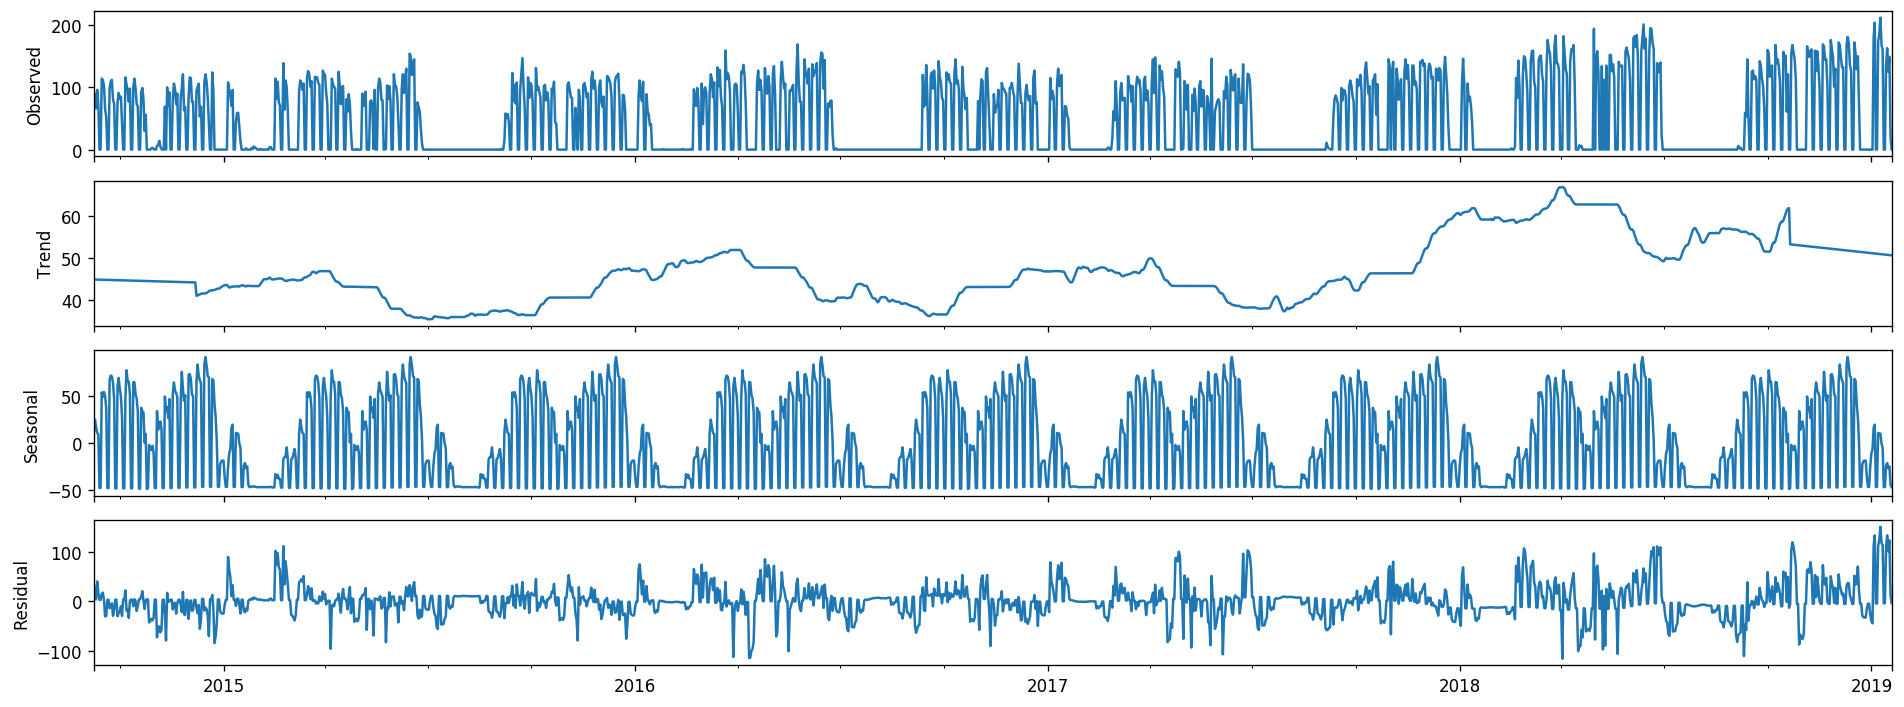
\includegraphics[width=\textwidth]{figures/seasonal_decompose_cafe.png}
	\caption{Décomposition de la série Café}
    \label{fig:seasonal_decompose_cafe}
\end{figure}

On remarque bien deux saisonnalités, l'une par semaine et l'autre par année.

Une fois la saisonalité observée, nous réalisons une recherche automatisée comme décrit précédemment \ref{par:grid_search} mais avec la composante saisonnale. Nous testons uniquement la périodicité par semaine $S=7$ car $S=182$ provoque un modèle trop coûteux.

Nous obtenons les résultats suivants.

\begin{table}[ht]
    \centering
    \begin{tabular}{r|l}
        AIC & 14127.09 \\
        BIC & 14164.00 \\
        MSE &  2249.31 \\
    \end{tabular}
    \caption{Résultats pour \SARIMA(1, 0, 0)(3, 0, 0, 7) sur le Café}
    \label{tab:pred_sarima_cafe}
\end{table}

\begin{figure}[ht]
    \centering
    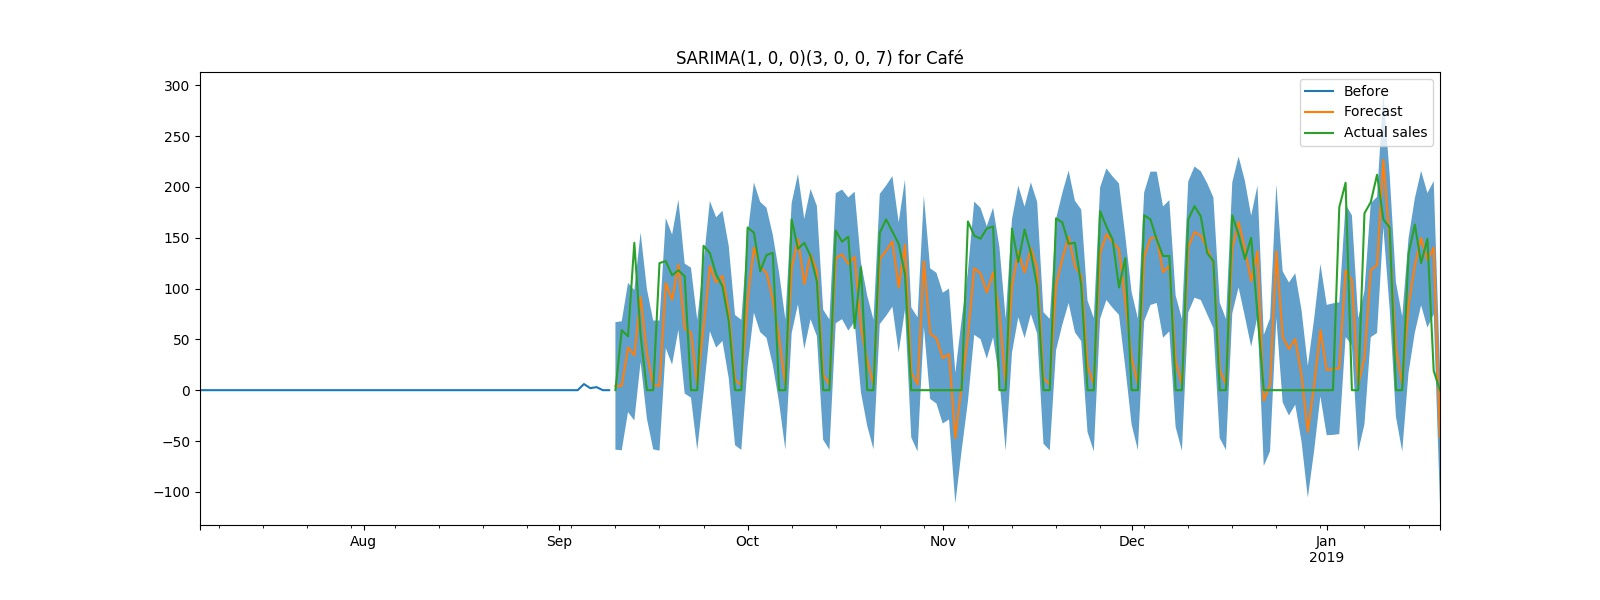
\includegraphics[width=\textwidth]{figures/pred_sarima_cafe.jpg}
    \caption{Prédiction \SARIMA pour le Café}
    \label{fig:pred_sarima_cafe}
\end{figure}

On ne note pas de grandes améliorations par rapport au modèle \ARIMA \ref{fig:pred_arima_cafe}. Il peut s'agir d'un problème de paramètres ou simplement que la saisonnalité n'est pas très intéressante.

Nous allons alors tenter d'ajouter des variables explicatives suivantes au modèle \SARIMAX.


\subsubsection{Le modèle \SARIMAX, ajout de variables exogènes}
\label{subsec:sarimax}

Afin de tenter d'améliorer les résultats du prédicteur, nous avons penser ajouter des variables explicatives telles que la présence de vacances ou d'examens.  Grâce au travail réalisé lors de la collecte des événements \ref{subsec:data_event}, cela est possible. Nous avons donc créé un DataFrame contenant les variables exogènes pour chaque jour:
\begin{itemize}[nolistsep]
    \item \code{weekly\_sin} et \code{weekly\_cos}: un encodage cyclique du numéro du jour dans la semaine
    \item \code{yearly\_sin} et \code{yearly\_cos}: un encodage cyclique du numéro de la semaine dans l'année
    \item \code{holiday}: la présence de vacances ou non en binaire
    \item \code{exams}: la présence d'examen ou non en binaire
    \item \code{weekofsemester}: le numéro de la semaine dans le semestre
\end{itemize}

L'encodage cyclique $f_P$ de période $P$ suit la fonction suivante:
\begin{equation}
    f_P(t) = \begin{pmatrix}
        \sin\left(\frac{2 \pi t}{P}\right) \\
        \cos\left(\frac{2 \pi t}{P}\right)
    \end{pmatrix}
    \label{eq:cycling_encoding}
\end{equation}

Ces variables nous semblaient intéressantes pour la prédiction, nous les avons testées et selectionnées.

Nous obtenons le DataFrame exogène suivant:
\begin{figure}[H]
    \centering
    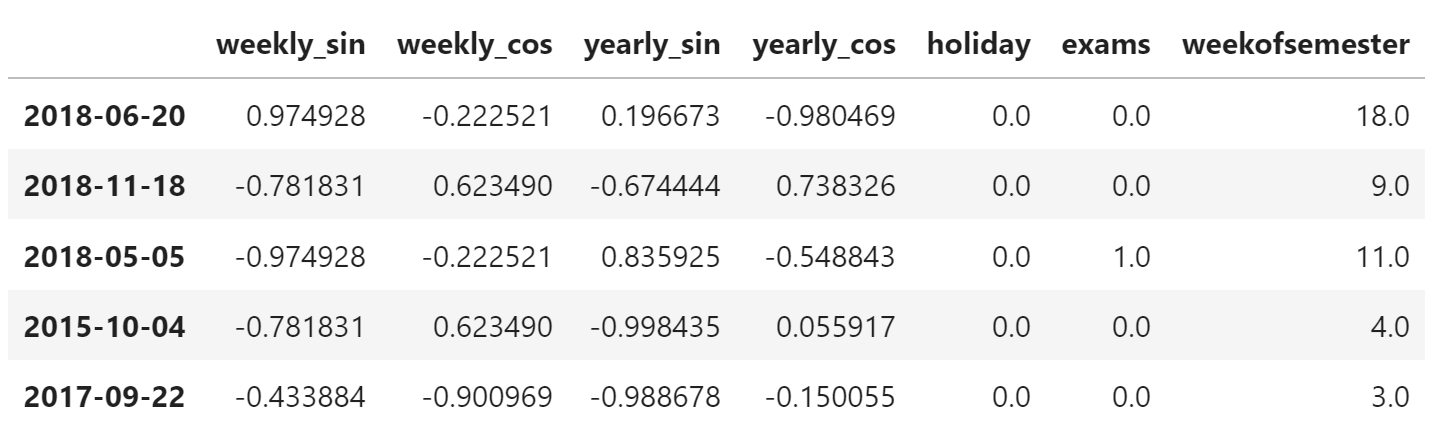
\includegraphics[width=\textwidth]{figures/exog_df.png}
    \caption{Aperçu du DataFrame des variables exogènes}
    \label{fig:exog_df}
\end{figure}

Nous testons alors cette configuration, et obtenons les résultats suivants.
\begin{table}[ht]
    \centering
    \begin{tabular}{r|l}
        AIC & 14259.78 \\
        \hline
        BIC & 14365.37 \\
        \hline
        MSE &  2015.17 \\
    \end{tabular}
    \caption{Résultats pour \SARIMAX(1, 0, 0)(3, 0, 0, 7) sur le Café}
    \label{tab:pred_sarimax_cafe}
\end{table}

\begin{figure}[ht]
    \centering
    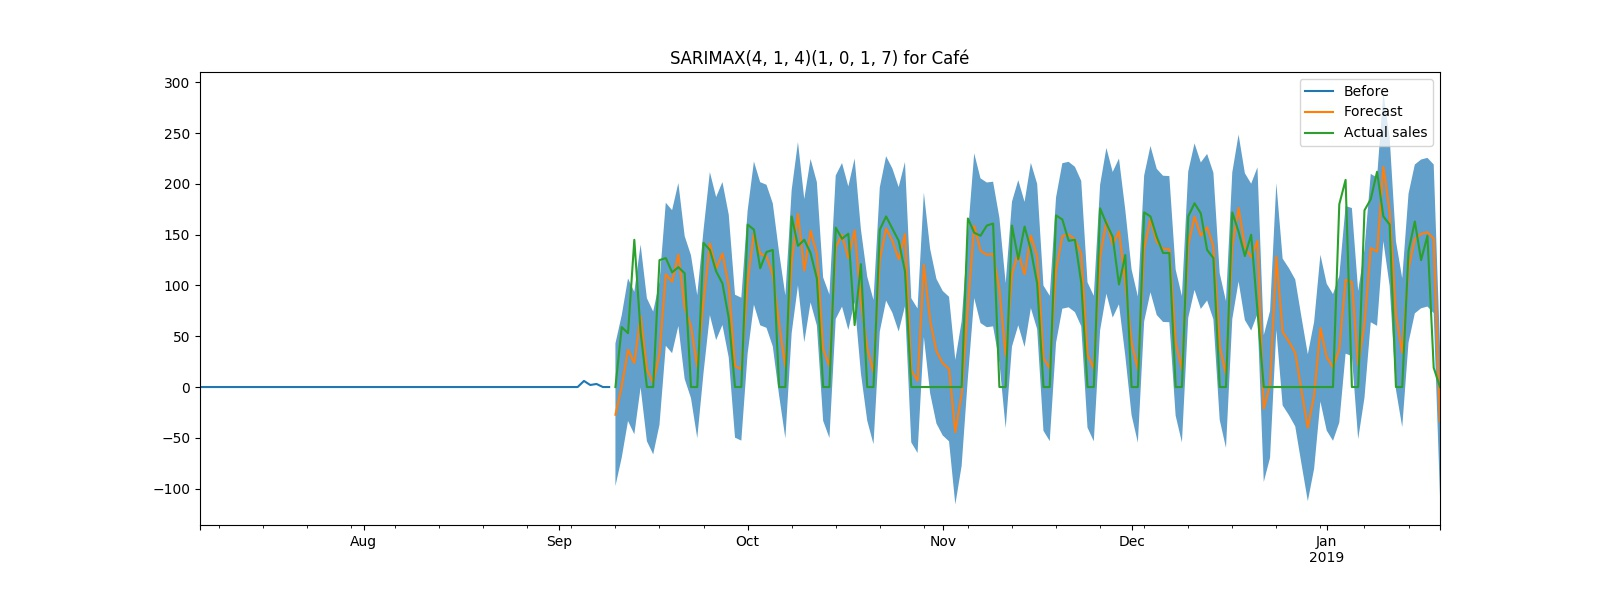
\includegraphics[width=\textwidth]{figures/pred_sarimax_cafe.jpg}
    \caption{Prédiction \SARIMAX pour le Café}
    \label{fig:pred_sarimax_cafe}
\end{figure}

On note une légère amélioration des résultats, on passe d'un MSE de $2401.85$ pour \ARIMA \ref{tab:pred_arima_cafe} à $2015.17$.

On s'aperçoit de plusieurs choses:
\begin{itemize}[nolistsep]
    \item les incertitudes sont toujours grandes
    \item des ventes négatives sont prédites alors que ce n'est pas possible
    \item la saisonnalité hebdomadaire est bien prise en compte
    \item l'évolution au cours du semestre semble juste
    \item les ventes sont trop basses
\end{itemize}

\SARIMAX a des difficultés avec les ventes nuls lors des jours où le pic est fermé. En réalité, nous avons l'impression que les variables exogènes améliorent un peu les prévisions mais on se rends rapidement compte que le problème général reste. En effet, en combinant de multiples variables, on peu s'approcher d'une prédiction correcte sur notre jeu de test mais cela ne permet en aucun cas de réaliser de bonnes prédictions: c'est de l'overfitting.


\subsection{Retour sur les bases et réflexions}
\label{subsec:back_to_basics}

Les prédictions semblent correctes mais comment les améliorer encore ?

\subsubsection{Décomposition de la tendance}
\label{subsec:decomp_trend}

Retournons à la base du modèle \ARIMA. Celui-ci fonctionne optimalement sur des séries stationnaires. Comment être sûr de la stationnarité de notre série ?

Repartons de la définition. Une série est dite stationnaire si son évolution ne dépends pas du temps. Notre série est composé d'une tendance, d'une saisonnalité et du "reste".

Dans un premier temps, il nous a paru évident que la tendance doit être étudiée à part. Elle fait évoluer la série en fonction du temps. Pour cela nous testons deux méthodes. La première, qui est la plus simple à mettre en place, consiste à soustraire la tendance de notre série et à traiter la série résultante. On utilise la décomposition 
comme vue précédemment et on enlève simplement la tendance. Ensuite on utilise un modèle \SARIMA sur la série sans tendance. Cela nous permettra de comprendre si le modèle fonctionne mieux dans le cas où la tendance est exclus car la série devrait être davantage stationnaire. 
Obtenant des résultats un peu meilleur visuellement, mais sans réelle quantification, nous avons appliqué une méthode plus réaliste, plus proche de l'état de production que pourrait avoir l'utilisation d'un tel modèle. Cela s'approche de l'utilisation des modèles en production, semaine par semaine.

Voici la méthode :
\begin{enumerate}
    \item Décomposition de la série avec 1 semestre de test et le reste pour l'entraînement.
    \item Séparation de la série d'entraînement en 2 séries distinctes, la tendance et le reste.
    \item Apprentissage du modèle \SARIMA sur la série d'entraînement sans tendance (les paramètres sont déterminés comme précédemment)
    \item Application d'un modèle de régression linéaire ou quadratique sur la tendance en fonction de sa forme.
    \item Prédiction du semestre suivant avec le modèle \SARIMA 
    \item Prédiction de la tendance avec le modèle de régression
    \item Assemblage des deux prédictions (par somme) et comparaison avec la série de test.
\end{enumerate}


Avec des résultats médiocres, on se demande si  il faut aussi enlever la partie saisonnal. Nous savons que les modèles ARIMA ne doivent pas comporter de saisonnalité mais les modèles SARIMA sont sensés palier ce problème. Nous avons quand même essayer la même démarche en enlevant la saisonnalité (grâce à la décomposition) et en utilisant les modèles ARIMA sur le reste, sans plus de résultats bien qu'il y est moins de paramètre à déterminer. 

\subsubsection{Transformation de la série temporelles}
\label{subsec:ts_remapping}

On s'intéresse à l'agencement de nos données, c'est-à-dire comment sont reparties les ventes sur les différents semestres. Voici un graphique détaillé de la répartition des semestres avec les vacances et les évènements, ainsi que des statistiques sur la durée des semestres.

\begin{figure}[ht]
	\centering
	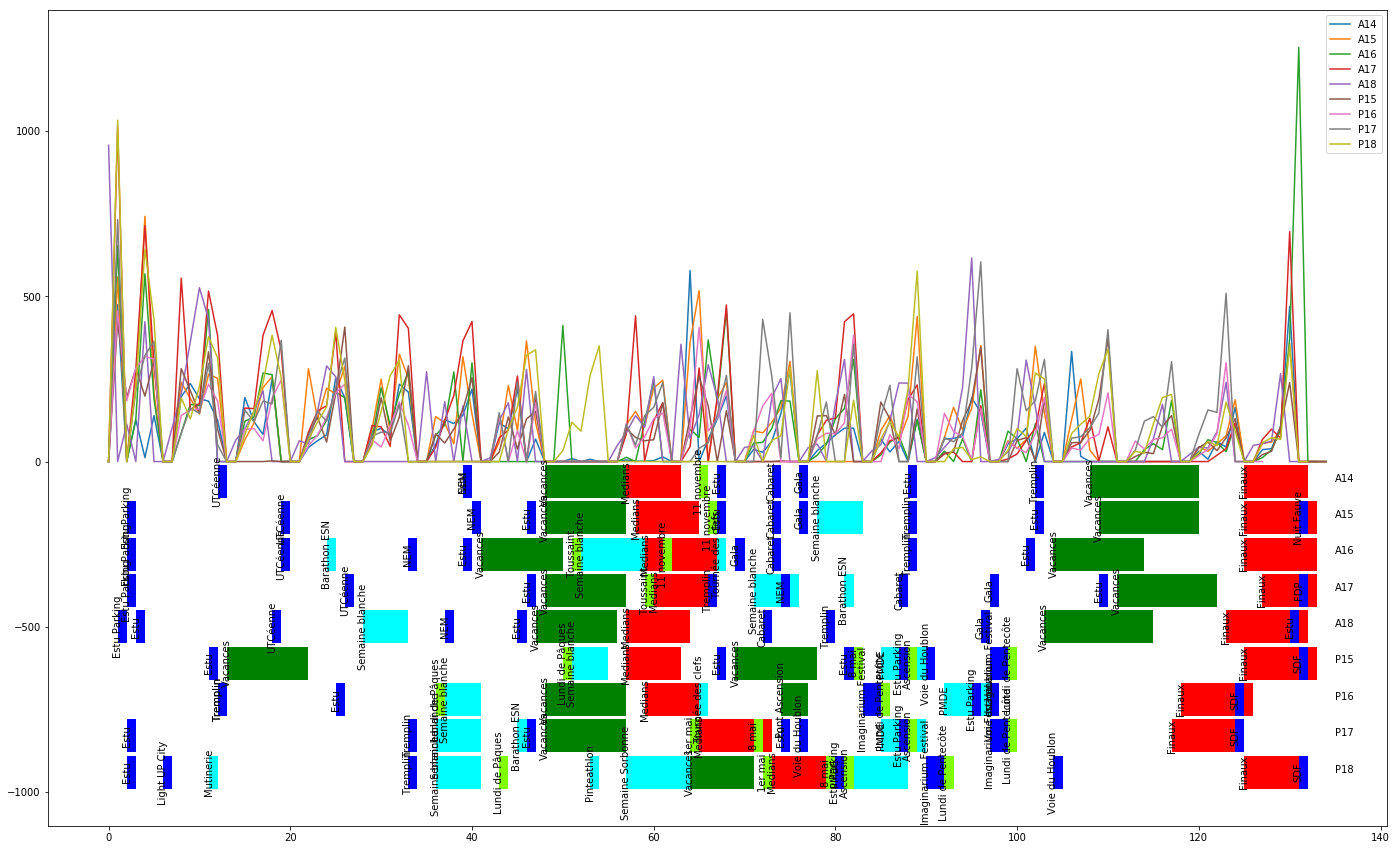
\includegraphics[width=1\textwidth]{figures/semester_sales_with_events.png}
	\caption{Visualisation de l'agencement des semestres}
    \label{fig:semester_events}
\end{figure}

\begin{table}[H]
    \centering
    \begin{tabular}{c|rr}
        \hline
        Semestre & Jours & Semaines \\
        \hline
        A14      &   133 &       19 \\
        A15      &   135 &       21 \\
        A16      &   135 &       21 \\
        A17      &   135 &       21 \\
        A18      &   132 &       19 \\
        P15      &   135 &       21 \\
        P16      &   128 &       20 \\
        P17      &   127 &       19 \\
        P18      &   133 &       20 \\
        \hline
        Moyenne  & 132.5 &     20.1
    \end{tabular}
    \caption{Statistiques sur la durée des semestres}
    \label{tab:semestre_days_stats}
\end{table}

Les semestres se ressemblent globalement mais ne sont pas identiques. Ils ne possèdent pas le même nombre de jours ni de semaines même si les écarts ne sont pas grands.

\paragraph{Reconstruction des semestres}

Avec les semestres d'Automne et de Printemps, nous avons deux types d'organisation. Nous avons deux périodes de vacances sur les semestres d'Automne et une seule sur les semestres de Printemps. Cela peut poser des problèmes pour la modélisation. Ce que l'on peut faire est de séparer notre problème en deux. On pourrait travailler avec deux modèles, un pour chaque type de semestre.

Pour le nombre de semaines pas exacte, on a plusieurs solutions: dans un premier temps, nous pouvons enlever les semaines en trop tant quelle ne sont pas trop près d'évènements tels que les vacances. On peut aussi penser à interpoler lorsque des semaines manquent ou dupliquer des semaines sans évènements.

En faisant cela, il nous reste à gérer le cas du placement des évènements. Nous pourrions transformer à la main tous les évènements des semestres afin qu'ils soient ordonnées similairement. Cela pose deux soucis majeurs. Le premier, qui est le moins grave est le temps nécessaire. Celui ci doit être fait pour chaque semestre lors de l'apprentissage et dois être de nouveau fait pour les semestres qui passent. Ensuite lors du travail à la main, il faudra interpoler et/ou enlever de nombreuses semaines afin d'avoir toujours exactement le même nombre de semaines entre chaque évènement.

Pour les week-ends nous faisons simple dès le début. Nous décidons de passer à la semaine de 5 jours et d'enlever les quelques ventes des samedis. Les vacances sont enlevées tout en réfléchissant aux positionnements des différentes semaines comme expliqué ci-dessus.

Nous pouvons imaginer une mise en production comme sur le diagramme si dessous: ("nous" correspond à l'apprentissage).
\begin{figure}[H]
	\centering
	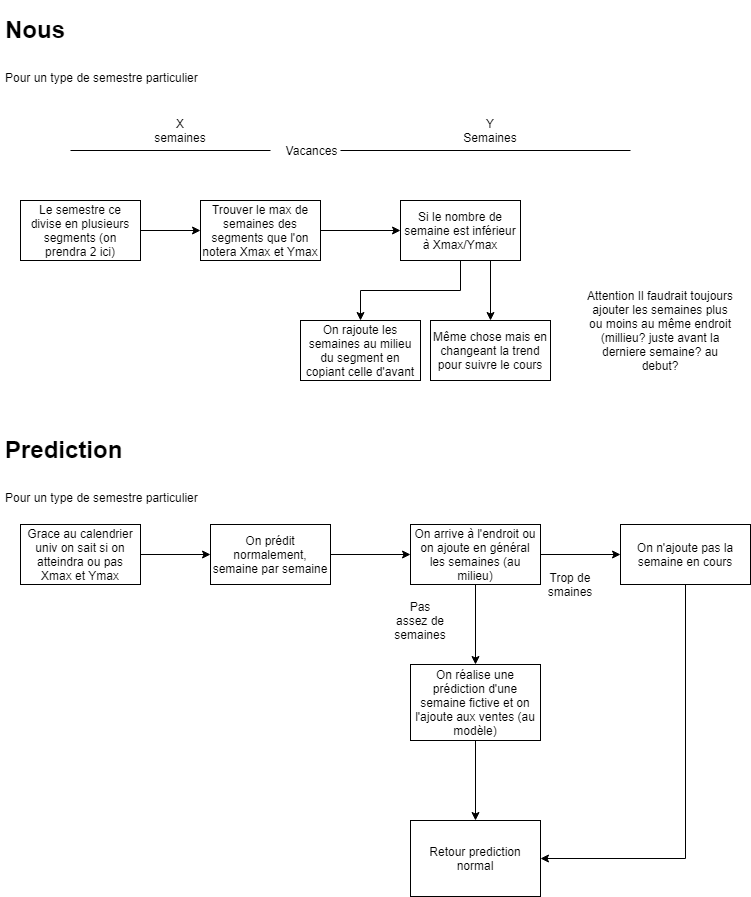
\includegraphics[width=1\textwidth]{figures/production.png}
	\caption{Schéma des transformation possibles des séries temporelles}
    \label{fig:scheme_remapping}
\end{figure}

Cependant cette solution est bien trop compliquée à mettre en place et à maintenir.
De plus nous ne sommes pas sûr de son efficacité. Manipuler les semaines poserait forcément des problèmes dans les prédictions et deviendrait vite ingérable.

\paragraph{Découpage des ventes nulles}

Les ventes sont souvent nulles (environ la moitié des observations) et tendent à fausser les modèles. Que se passe-t-il si nous retirons ces données ?

Nous avons créé la fonction \code{utils.datetime.remap\_ts} qui transforme la série selon la méthode suivante:
\begin{enumerate}[nolistsep]
    \item Passe les données des week-ends et des vacances à \code{NaN}
    \item Remplace les données des jours fériés par une moyenne du même jour des deux dernières semaines
\end{enumerate}

Cela permet d'enlever les données inintéressantes tout en conservant la série temporelle continue en temps.

Nous obtenons les résultats suivants:
\begin{table}[ht]
    \centering
    \begin{tabular}{r|l}
        AIC & 6507.99 \\
        \hline
        BIC & 6587.21 \\
        \hline
        MSE & 1239.62 \\
    \end{tabular}
    \caption{Résultats pour \SARIMAX(2, 0, 2)(0, 0, 1, 7) sur le ventes transformées de Café}
    \label{tab:pred_sarimax_cafe_remapped}
\end{table}

\begin{figure}[ht]
    \centering
    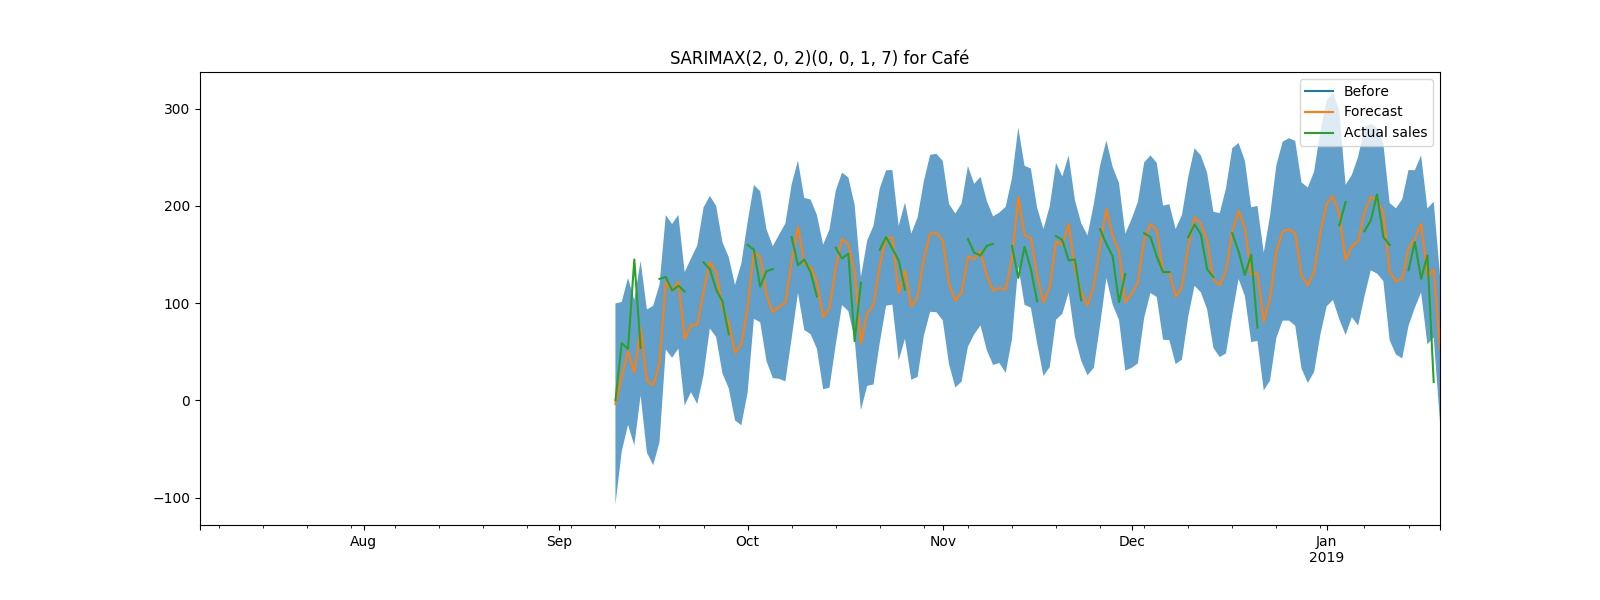
\includegraphics[width=\textwidth]{figures/pred_sarimax_cafe_remapped.jpg}
    \caption{Prédiction \SARIMAX(2, 0, 2)(0, 0, 1, 7) sur le ventes transformées de Café}
    \label{fig:pred_sarimax_cafe_remapped}
\end{figure}

On gagne significativement en AIC, BIC et MSE en les minimisant de moitié, mais aussi en rapidité, les valeurs \code{NaN} étant tout simplement passées.


\subsection{Comparaison des résultats}
\label{subsec:results_comparison}

En comparant les résultats \ref{tab:pred_arima_cafe}, \ref{tab:pred_sarima_cafe}, \ref{tab:pred_sarimax_cafe} et \ref{tab:pred_sarimax_cafe_remapped}, nous obtenons le classement suivant:

\begin{table}[H]
    \centering
    \begin{tabular}{r|rrrr}
        Indicateur & \ARIMA   & \SARIMA  & \SARIMAX & \SARIMAX transformé \\
        \hline
        AIC        & 14436.25 & 14127.09 & 14259.78 & 6507.99  \\
        BIC        & 14504.94 & 14164.00 & 14365.37 & 6587.21  \\
        MSE        &  2401.85 &  2249.31 &  2015.17 & 1239.62  \\
        Temps      &  8min24s & 17min13s & 46min54s & 18min43s \\
        \hline
        Classement & 4        & 2        & 3        & 1        \\
    \end{tabular}
    \caption{Comparaison des résultats}
    \label{tab:results_comparison}
\end{table}

Ainsi chaque étape de notre travail a permis d'améliorer les performances de prédictions. Le modèles \SARIMAX transformée \ref{fig:pred_sarimax_cafe_remapped} est le plus intéressant car plus précis que les autres tout en étant relativement rapide.

% \subsection{Comparaison avec d'autre types de modèles}

Dans le projet précédent, Sylvain Marchienne a réalisé lui aussi au préalable quelques recherches sur la prédiction des ventes. Il a par exemple utilisé le framework Prophet développé par Facebook. Prophet utilise une approche Bayésienne au problème de prédiction des séries temporelles. L'avantage principal de Prophet est sa facilité d'utilisation directement sur les données. En effet, celui-ci détermine lui-même automatiquement la tendance et la saisonnalité cachées dans la série. Cette simplicité et automatisation est à la fois son plus gros avantage mais aussi son plus grand défaut. En effet, si les prédictions ne sont pas à la hauteur, il devient très difficile d'en connaître la cause et encore plus compliqué de résoudre le problème. Les modèles \ARIMA nécessitent une évaluation des paramètres compliquée afin prendre en compte la saisonnalité par exemple mais sont plus robustes.

Les recherches faites par Sylvain sur Prophet et les différents modèles ne sont malheureusement que peu exploitable. En effet ceux ci ont été conçus sans aucune pensée pour la production. Ce sont des modèles à la semaine qui ne peuvent pas être comparé autrement que visuellement à nos modèles. De plus les tests sont réalisés sur des catégories de produits et non un produit en particulier. On s'attend, lorsque l'on réalise un modèle par semaines et par catégories de produits à visualiser moins d'erreurs. Ce n'est pas le cas et nos derniers modèles se comportent plutôt bien comparé aux modèles entraînés aux semestres précédents.

